\documentclass[fiche]{classe-tex3R} %#1=diapo (optionnel)
\usepackage{style-tex3R}
\usepackage{dirtree}
\parametrage

\colorlet{colorBasic}{SlateGrey}
\colorlet{colorBracket}{DarkViolet}
\colorlet{colorKeyword}{DarkBlue}
\colorlet{colorEnvironment}{LightSeaGreen}
\colorlet{colorComment}{Green}
\colorlet{colorString}{DarkOrange}
\colorlet{colorChange}{Red}
\colorlet{colorMath}{Teal}
\colorlet{colorVariable}{LightSkyBlue}
\colorlet{colorBoolean}{Indigo}
\colorlet{colorFunction}{DarkBlue}

\newcommand{\nocontentsline}[3]{}
\newcommand{\tocless}[2]{\bgroup\let\addcontentsline=\nocontentsline#1{#2}\egroup}

\lstset{
  %Réglages généraux
  backgroundcolor=\color{gray!20!white},
  basicstyle=\ttfamily\small\color{colorBasic},
  columns=fullflexible,
  aboveskip=0pt,
  belowskip=0pt,
  breaklines=true,
  %Keywords
  emph={[1]
    begin,
    end,
    documentclass,
    usepackage,
    definirchapitre,
    definirniveau,
    parametrage,
    bareme,
    competence,
    difficulte,
    source,
    theme,
    montitre,
    important,
    tailletexte,
    partie,
    souspartie,
    chapitre,
    visiblecmd,
    saut,
    lignes,
    ifdiapo,
    iffiche,
    ifheader,
    ifprint,
    ifactivite,
    ifbasique,
    ifbilan,
    ifcorrige,
    ifcours,
    ifTD,
    ifflash,
    ifDM,
    ifDS,
    ifinterro,
    ifcorrection,
    ifenonce,
    ifvisible,
    ifbareme,
    ifdifficulte,
    ifcompetence,
    ifsource,
    iftheme,
    ifstretch,
    ifsubfile,
    else,
    fi,
    newcounter,
    setcounter,
    stepcounter,
    thecompteurexercice,
    textbf,
    textit,
    underline,
    st,
    textsc,
    hl,
    mdseries,
    bfseries,
    itshape,
    scshape,
    huge,
    LARGE,
    Large,
    large,
    normalsize,
    small,
    footnotesize,
    scriptsize,
    tiny,
    color,
    textcolor,
    hspace,
    hfill,
    dotfill,
    vspace,
    vfill,
    newpage,
    item,
    task,
    renewcommand,
    arraystretch,
    rowcolors,
    hline,
    graphicspath,
    includegraphics,
    linewidth,
    textheight,
    adjustbox,
    fbox,
    rotatebox,
    reflectbox,
    scalebox,
    newline,
  }, 
  emphstyle={[1]\color{colorKeyword}},
  %Environnements
  emph={[2]
    environnement,
    luacode,
    fiche,
    document,
    application,
    convention,
    definition,
    exemple,
    methode,
    propriete,
    preuve,
    remarque,
    enonce,
    correction,
    visible,
    enumerate,
    itemize,
    tasks,
    tabular,
    minipage,
    align,
  }, 
  emphstyle={[2]\color{colorEnvironment}},
  %Variable lua
  emph={[3]
  Type,
  Impression,
  Header,
  Taille,
  Stretch,
  Correction,
  Enonce,
  Visible,
  Competence,
  Bareme,
  Difficulte,
  Source,
  Theme
  },
  emphstyle={[3]\color{colorVariable}},
  %Booléens lua
  emph={[4]
  true,
  false,
  nil
  },
  emphstyle={[4]\color{colorBoolean}},
  %Fonctions lua
  emph={[5]
  mesParametres
  },
  emphstyle={[4]\color{colorFunction}},
  %Literate
  literate={
    {\{}{{\textcolor{colorBracket}{\{}}}1
    {\}}{{\textcolor{colorBracket}{\}}}}1
    {[}{{\textcolor{colorBracket}{[}}}1
    {\&}{{\textcolor{colorBracket}{\& }}}1
    {]}{{\textcolor{colorBracket}{]}}}1
    {[[}{{\textcolor{colorString}{[[ }}}1
    {]]}{{\textcolor{colorString}{]]}}}1
    {\\}{{\textcolor{colorKeyword}{\textbackslash}}}1
    {..}{{\textcolor{colorMath}{\textbackslash}}}1
    % {0}{{$\cancel{0}$}}1
    },
  %Comment
  comment=[l]{--},
  morecomment=[l]{\%},
  commentstyle=\color{colorComment},
  %Delimiters
  moredelim=[is][\color{colorChange}]{@}{@},
  moredelim=[s][\color{colorMath}]{\$}{\$},
  moredelim=[s][\color{colorMath}]{\$\$}{\$\$},
  moredelim=[is][\color{colorMath}]{./}{./},
  moredelim=[is][\color{colorString}]{||}{||},
  moredelim=[is][\color{colorBasic}]{//}{//},
  moredelim=[is][\color{colorComment}]{/*}{/*},
  }


\title{\bfseries introduction basique à \LaTeX\par}
\author{Vincent Crombez \& Frédéric Léothaud}
\date{}

\cfoot{\pagemark}
\setlength{\parskip}{\baselineskip}
\setcounter{tocdepth}{3}
\renewcommand{\sectionformat}{\LARGE\textbf{\thesection~}}
  \setkomafont{section}{\normalfont\LARGE\color{Black}\bfseries}
\renewcommand{\subsectionformat}{\Large\textbf{\thesubsection~}}
  \setkomafont{subsection}{\normalfont\Large\color{Black}\bfseries}
\renewcommand{\subsubsectionformat}{\large\textbf{\thesubsubsection~}}
  \setkomafont{subsubsection}{\normalfont\large\color{Black}\bfseries}


\begin{document}

\maketitle

\newpage

\tableofcontents

\newpage

\phantomsection
\addcontentsline{toc}{section}{Introduction}
\section*{Introduction}

Avant de parler \LaTeX, il faut déjà avoir un éditeur et son compilateur associés qui fonctionnent. Plusieurs solutions s'ouvrent alors :

\begin{itemize}
  \item Utiliser un éditeur \textbf{en ligne} (\href{https://www.overleaf.com/}{Overleaf} est le plus populaire)
  \item Utiliser un éditeur \textbf{en local}, si l'installation n'est pas un vecteur de découragement.
\end{itemize}

L'installation d'un environnement local permet une plus grande souplesse et une meilleure personnalisation, mais peut parfois être source de stress et d'incompréhension. \href{https://github.com/Tex3rivieres/TeX3R-Portable}{\fbox{\faGithubSquare~TeX3R-Portable}} est une solution clé en main, basée sur des projets libres de droits, qui pourrait convenir à l'impatient. 

Les packages \href{https://ctan.mines-albi.fr/macros/latex/contrib/profcollege/doc/ProfCollege-doc.pdf}{\texttt{ProfCollege}} et \href{https://ctan.mines-albi.fr/macros/latex/contrib/scratch3/scratch3-fr.pdf}{\texttt{scratch3}} donnent des outils qui donnent envie de basculer vers \LaTeX, au moins partiellement (dans un premier temps \dots)

 \href{https://mirrors.ircam.fr/pub/CTAN/info/lshort/french/lshort-fr.pdf}{\textit{Une courte introduction à \LaTeX}} est un document un peu daté mais qui a le mérite d'être assez complet sur les bases du langage. 

 Ensuite, ce guide se veut plutôt comme un aide-mémoire des environnements basiques en \LaTeX.

 \section{Structure d'un document}

 \begin{lstlisting}
%Structure standard
\documentclass{//classe du document//} 
  
\usepackage{package1}
\usepackage{package2}   
...               
  
\begin{document}
//Corps du document //
...
\end{document}
  \end{lstlisting}
  
  \textbf{Note :} la classe par défaut en \LaTeX~ est la classe article. La classe TeX3R se base sur la classe KOMA-Script \texttt{scrartcl}. La classe TeX3R se veut complète et ne devrait pas nécessiter de chargement de packages supplémentaires la plupart du temps.

  \section{Police et taille}

  \adjustbox{valign=t}{\begin{minipage}{0.66\linewidth}%
      \begin{lstlisting}
%Package soul
Bonjour\\
\textbf{Bonjour}\\
\textit{Bonjour}\\
\underline{Bonjour}\\
\st{Bonjour}\\
\textsc{Bonjour}\\
\hl{Bonjour}
  \end{lstlisting}
  \end{minipage}}\hfill%
  \adjustbox{valign=t}{\begin{minipage}{0.3\linewidth}%
  Bonjour\\
  \textbf{Bonjour}\\
  \textit{Bonjour}\\
  \underline{Bonjour}\\
  \st{Bonjour}\\
  \textsc{Bonjour}\\
  \hl{Bonjour}
  \end{minipage}}%
  
\vspace{0pt}

  \adjustbox{valign=t}{\begin{minipage}{0.66\linewidth}%
     \begin{lstlisting}
{\mdseries Bonjour}\\
{\bfseries Bonjour}\\
{\itshape Bonjour}\\
{\scshape Bonjour}
     \end{lstlisting}
  \end{minipage}}\hfill%
  \adjustbox{valign=t}{\begin{minipage}{0.3\linewidth}%
     {\mdseries Bonjour}\\
  {\bfseries Bonjour}\\
  {\itshape Bonjour}\\
  {\scshape Bonjour} 
  \end{minipage}}%
  
  \vspace{0pt}

  \adjustbox{valign=t}{\begin{minipage}{0.66\linewidth}%
     \begin{lstlisting}
{\huge Bonjour}\\
{\LARGE Bonjour}\\
{\Large Bonjour}\\
{\large Bonjour}\\
{\normalsize Bonjour}\\
{\small Bonjour}\\
{\footnotesize Bonjour}\\
{\scriptsize Bonjour}\\
{\tiny Bonjour}   
     \end{lstlisting}
  \end{minipage}}\hfill%
  \adjustbox{valign=t}{\begin{minipage}{0.3\linewidth}%
     {\huge Bonjour}\\
     {\LARGE Bonjour}\\
     {\Large Bonjour}\\
     {\large Bonjour}\\
     {\normalsize Bonjour}\\
     {\small Bonjour}\\
     {\footnotesize Bonjour}\\
     {\scriptsize Bonjour}\\
     {\tiny Bonjour}      
  \end{minipage}}%

  \section{Couleur}

  \adjustbox{valign=t}{\begin{minipage}{0.66\linewidth}%
     \begin{lstlisting}
  %Package xcolor
  {\color{Red} Tout le texte en couleur rouge}
  
  Un mot en \textcolor{Green}{vert}
     \end{lstlisting}
  \end{minipage}}\hfill%
  \adjustbox{valign=t}{\begin{minipage}{0.3\linewidth}%
     %Package xcolor
  {\color{Red} Tout le texte en couleur rouge}
  
  Un mot en \textcolor{Green}{vert}
  \end{minipage}}%
  
  \textbf{Note :} On peut utiliser les codes RGB, HTML ou définir ses propres couleurs (voir  \href{https://ctan.mines-albi.fr/macros/latex/contrib/xcolor/xcolor.pdf}{documentation de \texttt{xcolor} sur CTAN}). Pour la plupart des usages courants, la table ci-dessous suffit :
  
  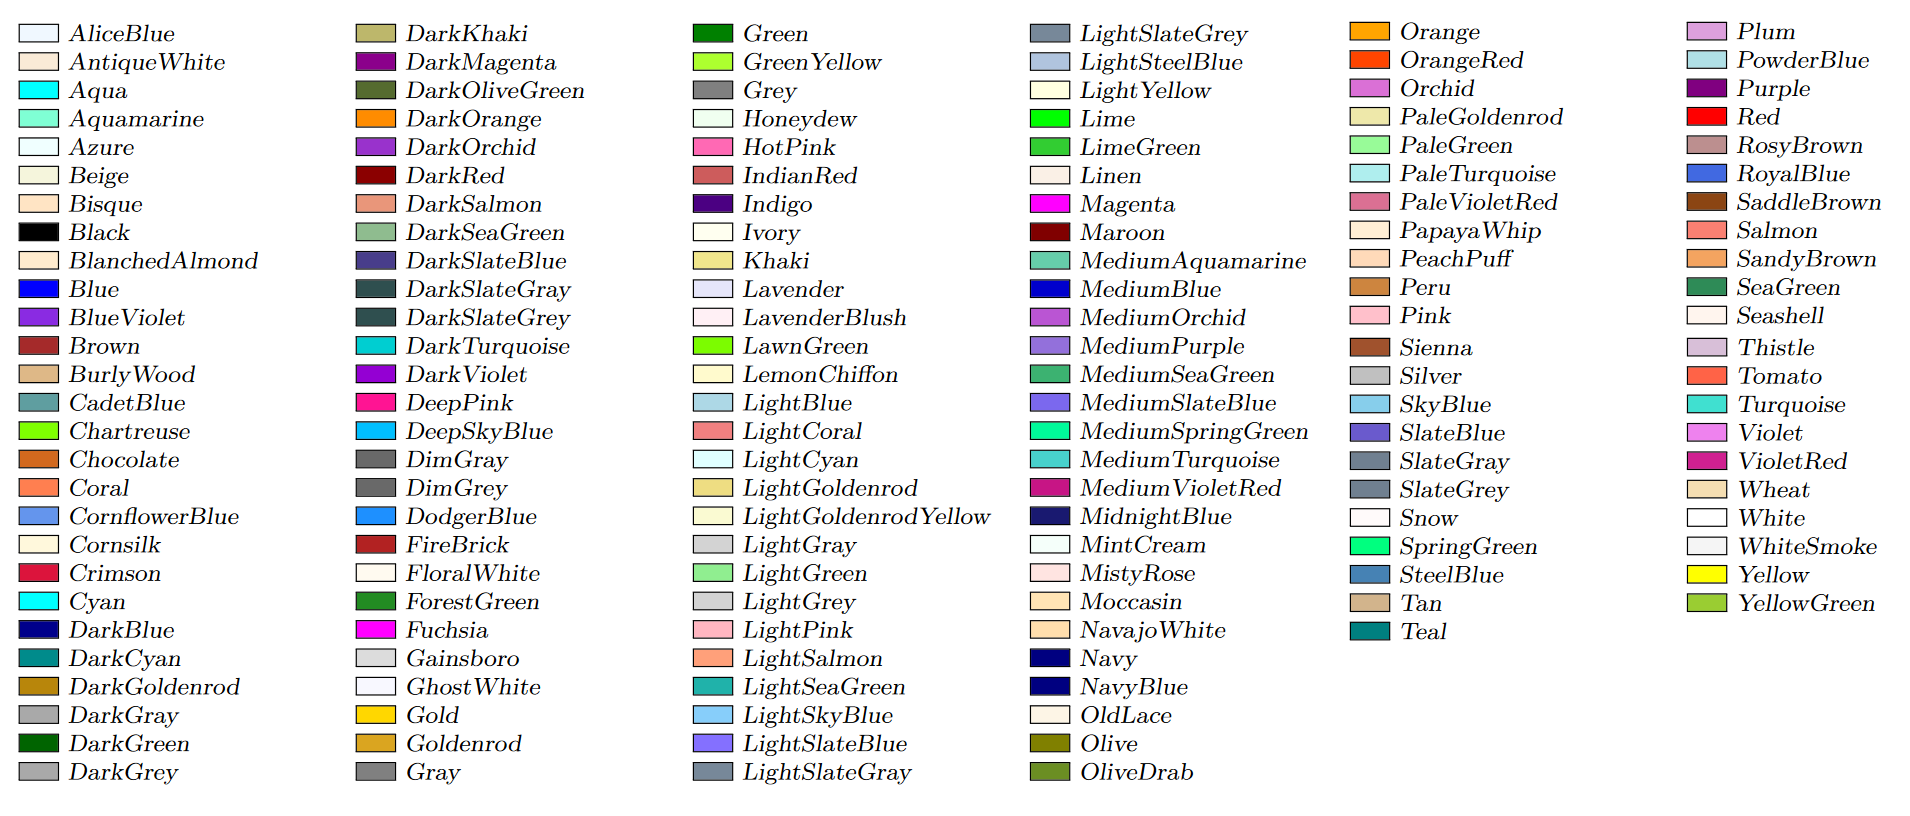
\includegraphics[width=1\linewidth]{Couleurs.png}


  \section{Espacement}

\adjustbox{valign=t}{\begin{minipage}{0.48\linewidth}%
   \begin{lstlisting}[escapeinside=||]
%Espaces horizontaux
a~b\\ %Espace insécable
a\,b\\ %Espace fin
a\hspace{3cm} b\\ %Espace de valeur fixe
a\hfill b\\ %Remplit l'espace
a\dotfill b %Remplit l'espace de pointillés
   \end{lstlisting}
\end{minipage}}\hfill%
\adjustbox{valign=t}{\begin{minipage}{0.48\linewidth}%
a~b\\ %Espace insécable
a\,b\\ %Espace fin
a\hspace{3cm} b\\ %Espace de valeur fixe
a\hfill b\\ %Remplit l'espace
a \dotfill b %Remplit l'espace de pointillés
\end{minipage}}%

\vspace{0pt}

\adjustbox{valign=t}{\begin{minipage}{0.48\linewidth}%
\begin{lstlisting}
%Trois manières différentes de marquer un saut de ligne
a\\b

c\newline d

e

f

%Marquer un changement de paragraphe 
g\par h
\end{lstlisting}
\end{minipage}}\hfill%
\adjustbox{valign=t}{\begin{minipage}{0.48\linewidth}%
   %Trois manières différentes de marquer un saut de ligne
   a\\b
   
   c\newline d
   
   e

   f

   %Marquer un changement de paragraphe 
   g\par h
\end{minipage}}%

\vspace{0pt}

\adjustbox{valign=t}{\begin{minipage}{0.48\linewidth}%
   \begin{lstlisting}
%Espaces verticaux

\vspace*{1cm}%Valeur fixe en haut de page

a

%Valeur fixe
b

\vspace{3cm}

c

%Saut d'une valeur fixe d'une ligne
d

e

%Remplit l'espace vertical (ne marche pas dans une minipage)
f

\vfill

g
   \end{lstlisting}
\end{minipage}}\hfill%
\adjustbox{valign=t}{\begin{minipage}{0.48\linewidth}%
   \vspace*{0.5cm}%Valeur fixe en haut de page

a

%Valeur fixe
b

\vspace{1cm}

c

%Saut d'une valeur fixe d'une ligne
d

e

%Remplit l'espace vertical (ne marche pas dans une minipage)
f

\vspace{7cm}

g
\end{minipage}}%

\saut{ligne}

\begin{lstlisting}
%Saut de page
\newpage
\end{lstlisting}

\section{Listes et énumérations}

\adjustbox{valign=t}{\begin{minipage}{0.48\linewidth}%
\begin{lstlisting}
\begin{enumerate}
  \item Premier
  \item Deuxième
  \item Troisième
\end{enumerate}
\end{lstlisting}
\end{minipage}}\hfill%
\adjustbox{valign=t}{\begin{minipage}{0.48\linewidth}%
   \begin{enumerate}
    \item Premier
    \item Deuxième
    \item Troisième
   \end{enumerate}
\end{minipage}}\par

\vspace{0pt}

\adjustbox{valign=t}{\begin{minipage}{0.48\linewidth}%
\begin{lstlisting}
\begin{itemize}
  \item Premier
  \item Deuxième
  \item Troisième
\end{itemize}
\end{lstlisting}
\end{minipage}}\hfill%
\adjustbox{valign=t}{\begin{minipage}{0.48\linewidth}%
   \begin{itemize}
    \item Premier
    \item Deuxième
    \item Troisième
   \end{itemize}
\end{minipage}}\par

\vspace{0pt}

\adjustbox{valign=t}{\begin{minipage}{0.48\linewidth}%
   \begin{lstlisting}
\begin{enumerate}
  \setcounter{enumi}{2}
  \item Troisième
  \item Quatrième
  \item Cinquième
\end{enumerate}
   \end{lstlisting}
\end{minipage}}\hfill%
\adjustbox{valign=t}{\begin{minipage}{0.48\linewidth}%
   \begin{enumerate}
  \setcounter{enumi}{2}
  \item Troisième
  \item Quatrième
  \item Cinquième
\end{enumerate}
\end{minipage}}\par

\vspace{0pt}

\adjustbox{valign=t}{\begin{minipage}{0.48\linewidth}%
   \begin{lstlisting}
%Package tasks
\begin{tasks}[style=itemize](3)
  \task Premier
  \task Deuxième
  \task Troisième
  \task Quatrième
  \task Cinquième 
  \task Sixième
\end{tasks}   
   \end{lstlisting}
\end{minipage}}\hfill%
\adjustbox{valign=t}{\begin{minipage}{0.48\linewidth}%
  \begin{tasks}[style=itemize](3)
    \task Premier
    \task Deuxième
    \task Troisième
    \task Quatrième
    \task Cinquième 
    \task Sixième
\end{tasks}
\end{minipage}}\par

\vspace{0pt}

\adjustbox{valign=t}{\begin{minipage}{0.48\linewidth}%
\begin{lstlisting}
%Package tasks
\begin{tasks}[//style=enumerate//](2)
  \task Premier
  \task Deuxième
  \task* Troisième vraiment beaucoup beaucoup trop long
  \task Quatrième
  \task Cinquième 
\end{tasks}
\end{lstlisting}   
\end{minipage}}\hfill%
\adjustbox{valign=t}{\begin{minipage}{0.48\linewidth}%
  \begin{tasks}[style=enumerate](2)
  \task Premier
  \task Deuxième
  \task* Troisième vraiment beaucoup beaucoup trop long
  \task Quatrième
  \task Cinquième 
\end{tasks}
\end{minipage}}\par

\vspace{0pt}

\adjustbox{valign=t}{\begin{minipage}{0.48\linewidth}%
   \begin{lstlisting}
%Package enumitem
\begin{enumerate}
  \item Premier
  \item Deuxième
\end{enumerate}

Une phrase.

\begin{enumerate}[resume]
  \item Troisième
  \item Quatrième
\end{enumerate}
   \end{lstlisting}
\end{minipage}}\hfill%
\adjustbox{valign=t}{\begin{minipage}{0.48\linewidth}%
  \begin{enumerate}
    \item Premier
    \item Deuxième
  \end{enumerate}

  Une phrase.

  \begin{enumerate}[resume]
    \item Troisième
    \item Quatrième
  \end{enumerate}  
\end{minipage}}%

\section{Tableaux}

\adjustbox{valign=t}{\begin{minipage}{0.48\linewidth}%
   \begin{lstlisting}
\begin{tabular}{l|r|c|p{4cm}|}
  Cell. 1 & Cell. 2 & Cell. 3 & Cell. 4\\
  \hline
  Cell. 5 & Cell. 6 & Cell. 7 & Cell. 8\\
\end{tabular}
   \end{lstlisting}
\end{minipage}}\hfill%
\adjustbox{valign=t}{\begin{minipage}{0.48\linewidth}%
   \begin{tabular}{l|r|c|p{4cm}|}
  Cell. 1 & Cell. 2 & Cell. 3 & Cell. 4\\
  \hline
  Cell. 5 & Cell. 6 & Cell. 7 & Cell. 8\\
\end{tabular}
\end{minipage}}\par

\vspace{0pt}

\adjustbox{valign=t}{\begin{minipage}{0.48\linewidth}%
   \begin{lstlisting}
\renewcommand{\arraystretch}{2}
\begin{tabular}{l|r|c|p{4cm}|}
  Cell. 1 & Cell. 2 & Cell. 3 & Cell. 4\\
  \hline
  Cell. 5 & Cell. 6 & Cell. 7 & Cell. 8\\
\end{tabular}
   \end{lstlisting}
\end{minipage}}\hfill%
\adjustbox{valign=t}{\begin{minipage}{0.48\linewidth}%
  \renewcommand{\arraystretch}{2}
  \begin{tabular}{l|r|c|p{4cm}|}
  Cell. 1 & Cell. 2 & Cell. 3 & Cell. 4\\
  \hline
  Cell. 5 & Cell. 6 & Cell. 7 & Cell. 8\\
\end{tabular}
\end{minipage}}\par

\vspace{0pt}

\adjustbox{valign=t}{\begin{minipage}{0.48\linewidth}%
   \begin{lstlisting}
%Package xcolor et colortbl
\rowcolors{1}{gray!20}{white}
\begin{tabular}{c|c}%l|c|r|p{1cm}
  Cellule 1 & Cellule 2\\ 
  Cellule 3 & Cellule 4\\
  Cellule 5 & Cellule 6\\
  Cellule 7 & Cellule 8\\
\end{tabular}
   \end{lstlisting}
\end{minipage}}\hfill%
\adjustbox{valign=t}{\begin{minipage}{0.48\linewidth}%
  %Package xcolor et colortbl
\rowcolors{1}{gray!20}{white}
\begin{tabular}{c|c}%l|c|r|p{1cm}
  Cellule 1 & Cellule 2\\ 
  Cellule 3 & Cellule 4\\
  Cellule 5 & Cellule 6\\
  Cellule 7 & Cellule 8\\
\end{tabular}
\end{minipage}}%

\textbf{Outil de génération de tableaux :} \url{https://www.tablesgenerator.com/#}



\section{Images}

\textbf{Note :} l'image doit être à la racine du document ou le chemin vers l'image doit être spécifié via la commande \verb!\graphicspath! ou dans les options de \verb!\includegraphics!

\adjustbox{valign=t}{\begin{minipage}{0.48\linewidth}%
   \begin{lstlisting}
%Package graphicx
%Ces commandes insérent correctement les images situées dans l'arborescence ci-contre
\graphicspath{{./Images/}}

\includegraphics{image1.png}
\includegraphics{image2}
\includegraphics{./Autres/image3.pdf}
\includegraphics{image4}
   \end{lstlisting}

\end{minipage}}\hfill%
\adjustbox{valign=t}{\begin{minipage}{0.48\linewidth}%
   \dirtree{%
   .1 Mon dossier.
   .2 Images.
   .3 image1.png.
   .3 image2.jpg.
   .2 Autres.
   .3 image3.pdf.
   .2 Mon fichier.tex.
   .2 image4.gif.
   }
\end{minipage}}%

\saut{ligne}

\begin{lstlisting}
%Voici différentes options d'insertion d'image :

\includegraphics{image1} %Taille réelle
\includegraphics[scale=0.75]{image1}%0.75 x taille réelle 
\includegraphics[width=5cm]{image1} %Largeur fixe
\includegraphics[width=\linewidth]{image1} %S'adapte à la largeur de la ligne
\includegraphics[height=3cm]{image1}%Hauteur fixe
\includegraphics[height=0.8\textheight]{image1}%0.80 x Hauteur de la zone de texte actuelle
\end{lstlisting}


\section{Minipages et boîtes}

\adjustbox{valign=t}{\begin{minipage}{0.48\linewidth}%
   \begin{lstlisting}
\begin{minipage}{0.48\linewidth}%
   Première colonne
\end{minipage}\hfill%
\begin{minipage}{0.48\linewidth}%
   Deuxième colonne
\end{minipage}%
   \end{lstlisting}
\end{minipage}}\hfill%
\adjustbox{valign=t}{\begin{minipage}{0.48\linewidth}%
  \begin{minipage}{0.48\linewidth}%
   Première colonne
\end{minipage}\hfill%
\begin{minipage}{0.48\linewidth}%
   Deuxième colonne
\end{minipage}%
\end{minipage}}\par

\vspace{0pt}

\adjustbox{valign=t}{\begin{minipage}{0.48\linewidth}%
   \begin{lstlisting}
\begin{minipage}{0.32\linewidth}%
   Première colonne
\end{minipage}\hfill%
\begin{minipage}{0.32\linewidth}%
   Deuxième colonne
\end{minipage}\hfill%
\begin{minipage}{0.32\linewidth}%
   Troisième colonne
\end{minipage}%
   \end{lstlisting}
\end{minipage}}\hfill%
\adjustbox{valign=t}{\begin{minipage}{0.48\linewidth}%
  \begin{minipage}{0.32\linewidth}%
   Première colonne
\end{minipage}\hfill%
\begin{minipage}{0.32\linewidth}%
   Deuxième colonne
\end{minipage}\hfill%
\begin{minipage}{0.32\linewidth}%
   Troisième colonne
\end{minipage}%
\end{minipage}}%

\vspace{0pt}

\adjustbox{valign=t}{\begin{minipage}{0.48\linewidth}%
\begin{lstlisting}
\begin{minipage}{0.48\linewidth}%
   Première colonne plus grande
\end{minipage}\hfill%
\begin{minipage}{0.24\linewidth}%
   Deuxième colonne
\end{minipage}\hfill%
\begin{minipage}{0.24\linewidth}%
   Troisième colonne
\end{minipage}%
\end{lstlisting}
\end{minipage}}\hfill%
\adjustbox{valign=t}{\begin{minipage}{0.48\linewidth}%
  \begin{minipage}{0.48\linewidth}%
    Première colonne plus grande
  \end{minipage}\hfill%
  \begin{minipage}{0.24\linewidth}%
    Deuxième colonne
  \end{minipage}\hfill%
  \begin{minipage}{0.24\linewidth}%
    Troisième colonne
  \end{minipage}%
\end{minipage}}%



\textbf{Note :} la commande \textbackslash adjustbox permet de régler de nombreux problèmes d'alignement.

\adjustbox{valign=t}{\begin{minipage}{0.48\linewidth}%
   \begin{lstlisting}
\adjustbox{valign=t}{\begin{minipage}{0.48\linewidth}%
   Du texte à gauche d'une image, qui peut s'étendre sur plusieurs lignes.
\end{minipage}}\hfill%
\adjustbox{valign=t}{\begin{minipage}{0.48\linewidth}%
   \includegraphics[width=\linewidth]{example-image-a}
\end{minipage}}%
   \end{lstlisting}
\end{minipage}}\hfill%
\adjustbox{valign=t}{\begin{minipage}{0.48\linewidth}%
   \adjustbox{valign=t}{\begin{minipage}{0.48\linewidth}%
   Du texte à gauche d'une image, qui peut s'étendre sur plusieurs lignes.
  \end{minipage}}\hfill%
  \adjustbox{valign=t}{\begin{minipage}{0.48\linewidth}%
    \includegraphics[width=\linewidth]{example-image-a}
  \end{minipage}}%
\end{minipage}}%

\vspace{0pt}

\adjustbox{valign=t}{\begin{minipage}{0.48\linewidth}%
   \begin{lstlisting}
Ceci est une 
\begin{minipage}{3.2cm}
   Je suis un texte en plein milieu de la phrase.
\end{minipage} 
phrase bizarre.
   \end{lstlisting}
\end{minipage}}\hfill%
\adjustbox{valign=t}{\begin{minipage}{0.48\linewidth}%
   Ceci est une 
      \begin{minipage}{3.2cm}
      Je suis un texte en plein milieu de la phrase.
      \end{minipage} 
   phrase bizarre.
\end{minipage}}%

\vspace{0pt}

\adjustbox{valign=t}{\begin{minipage}{0.48\linewidth}%
   \begin{lstlisting}
Ceci est une 
\fbox{
   \begin{minipage}[c]{3.2cm}
      Je suis un texte en plein milieu de la phrase.
   \end{minipage}
} 
phrase bizarre.
\end{lstlisting}
\end{minipage}}\hfill%
\adjustbox{valign=t}{\begin{minipage}{0.48\linewidth}%
  Ceci est une 
\fbox{
   \begin{minipage}[c]{3.2cm}
      Je suis un texte en plein milieu de la phrase.
   \end{minipage}
} 
phrase bizarre. 
\end{minipage}}%

\vspace{0pt}

\adjustbox{valign=t}{\begin{minipage}{0.48\linewidth}%
   \begin{lstlisting}
Ceci est une 
\rotatebox[origin=c]{45}{
   \begin{minipage}[c]{3.2cm}
      Je suis un texte en plein milieu de la phrase.
   \end{minipage}
} 
phrase bizarre.
\end{lstlisting}
\end{minipage}}\hfill%
\adjustbox{valign=t}{\begin{minipage}{0.48\linewidth}%
   Ceci est une 
\rotatebox[origin=c]{45}{
   \begin{minipage}[c]{3.2cm}
      Je suis un texte en plein milieu de la phrase.
   \end{minipage}
} 
phrase bizarre.
\end{minipage}}%

\vspace{0pt}

\adjustbox{valign=t}{\begin{minipage}{0.48\linewidth}%
   \begin{lstlisting}
Ceci est une 
\reflectbox{
   \begin{minipage}[c]{3.2cm}
      Je suis un texte en plein milieu de la phrase.
   \end{minipage}
} 
phrase bizarre.
   \end{lstlisting}
\end{minipage}}\hfill%
\adjustbox{valign=t}{\begin{minipage}{0.48\linewidth}%
Ceci est une 
\reflectbox{
   \begin{minipage}[c]{3.2cm}
      Je suis un texte en plein milieu de la phrase.
   \end{minipage}
} 
phrase bizarre.
\end{minipage}}%

\vspace{0pt}

\adjustbox{valign=t}{\begin{minipage}{0.48\linewidth}%
  \begin{lstlisting}
Ceci est une 
\scalebox{0.5}{
  \begin{minipage}[c]{3.2cm}
     Je suis un texte en plein milieu de la phrase.
  \end{minipage}
} 
phrase bizarre.
  \end{lstlisting}
\end{minipage}}\hfill%
\adjustbox{valign=t}{\begin{minipage}{0.48\linewidth}%
Ceci est une 
\scalebox{0.5}{%
  \begin{minipage}[c]{3.2cm}
     Je suis un texte en plein milieu de la phrase.
  \end{minipage}
} 
phrase bizarre.
\end{minipage}}%


\section{Math mode}

\adjustbox{valign=t}{\begin{minipage}{0.48\linewidth}%
\begin{lstlisting}
$4x+5=12x-8$

$$8x-3=5x+2$$

\begin{align*}
   ./A./ & ./=(5x+3)(2x-5)./\\
     &./ = 10x^2-19x-15./
\end{align*}
\end{lstlisting}
   

\end{minipage}}\hfill%
\adjustbox{valign=t}{\begin{minipage}{0.48\linewidth}%
$4x+5=12x-8$

$$8x-3=5x+2$$

\begin{align*}
   A & =(5x+3)(2x-5)\\
     & = 10x^2-19x-15
\end{align*}
\end{minipage}}%

\vspace{0pt}

\adjustbox{valign=t}{\begin{minipage}{0.48\linewidth}%
\begin{lstlisting}
$..dfrac{35}{21}=..dfrac{..cancel{7}..times 5}{..cancel{7}..times 3}=..dfrac{5}{3}$

$$f(x)=7..left(..dfrac{1}{5} + 2x..right)$$

$..mathcal{A}_..text{triangle}=..dfrac{\text{base}..times..text{hauteur}}{2}$
\end{lstlisting}
\end{minipage}}\hfill%
\adjustbox{valign=t}{\begin{minipage}{0.48\linewidth}%
   $\dfrac{35}{21}=\dfrac{\cancel{7}\times 5}{\cancel{7}\times 3}=\dfrac{5}{3}$

   $$f(x)=7\left(\dfrac{1}{5} + 2x\right)$$

   $\mathcal{A}_\text{triangle}=\dfrac{\text{base}\times\text{hauteur}}{2}$
\end{minipage}}%

\textbf{Note :} les commandes d'espacement ne fonctionnent pas en math-mode, en dehors de la commande \verb!\text!

\end{document}